\documentclass[../diploma.tex]{subfiles}
\begin{document}\label{sec:3}

Данная глава посвящена сравнению описанных выше стратегий. В ней описывается подготовка необходимых тестовых данных, приведены результаты экспериментов с применением стратегий на этих данных, и сделаны соответствующие выводы.

\subsection{Подготовка тестовых данных}\label{dataset}

Тестовые данные для этой работы состоят из двух частей. Первая, синтетическая, была написана специально для этой работы и представляет из себя несколько наборов функций, в каждом из которой размер и сложность функций равномерно увеличивается по заданному шаблону. Вторая часть взята из реальной практики верификации смарт-контрактов.

Для того, чтобы синтетические данные подходили для численных экспериментов, необходимо было создать логически несложный код, который может повторяться с незначительными изменениями неограниченное число раз. Вместе с этим необходимо было протестировать такие фундаментальные элементы языков программирования, как условные переходы и рекурсия. В то же время циклы не были включены в этот код, поскольку верификация кода с циклами является отдельной областью исследований, ставящих множество уникальных вопросов \cite{loops_are_hard}, и выходит за рамки этой работы.

Для построения синтетических тестовых данных был выбран классический алгоритм подсчёта полиномиального хеша строки. Этот алгоритм был реализован на языке Ursus в различных вариациях. При этом для этих алгоритмов верифицируется соответствие реализации референсной реализации на языке Coq. Синтетический набор состоит из следующих наборов функций:

\begin{itemize}
    \item \textbf{Simple}. $i$-я функция вычисляет хеш первых $i$ символов строки, при этом код является линейным (не использует циклы или рекурсию), то есть размер кода линейно зависит от порядкового номера функции.
    \item \textbf{If}. Расширение набора \textbf{Simple}, в котором симулируется работа с нуль-\\ терминированными строками. В случае, если программа дошла до нулевого символа, вычисление должно завершиться. Этот набор позволяет протестировать условный оператор и досрочный выход из функции.
    \item \textbf{Recursion}. Рекурсивная версия набора \textbf{Simple}. В ней функция с номером $i+1$ сначала вызывает функцию $i$, а затем дополняет вычисление $(i+1)$-м символом.
    \item \textbf{IfAndRecursion}. Рекурсивная версия набора \textbf{If}.
\end{itemize}

Для реальной части тестовых данных был выбран кошелек с мультиподписью из экосистемы TON \cite{multisig}. Кошельки с мультиподписью используются в блокчейн-сетях повсеместно \cite{wallets_survey} и являются критическим элементом для безопасности многих систем, поэтому верификация таких кошельков имеет практическую значимость. Материалы для верификации этого смарт-контракта были взяты из практики компании Pruvendo, в том числе трансляция кода с исходного языка Solidity на Ursus и формальная спецификация этой системы. Эксперименты заключались в применении разных стратегий для доказательства имеющейся формальной спецификации.

Все эксперименты поставлены на процессоре Intel Xeon E5-2687W v4 @ 3.00GHz с 512 Гб оперативной памяти и 48 ядрами, использовалась версия Coq 8.16.1.

\subsection{Эксперименты на синтетических данных}

Начнём сравнение стратегий с выявления наименее производительных стратегий, которые определённо не подходят к применению на практике, поскольку работают относительно долго даже на тестах небольшое размеров. Такими стратегиями являются все стратегии, основанные на базовых стратегиях \texttt{bottomup-naive} и \texttt{bottomup-reductions}. На рисунке \ref{plot_bottomup} приведены результаты этих стратегий на наборе тестов Simple. Тогда как стратегия \texttt{native-lazy}, приведённая на этих графиках для сравнения, вычисляет систему уравнений размера 10 за минуту, вычисления для \texttt{bottomup-naive} во всех вариациях и со всеми оптимизациями не укладываются в пять минут на тесте размера 4, а для \texttt{bottomup-reductions}~--- уже на тесте размера 2. На этих и дальнейших графиках вычисления ограничены пятью минутами, то есть измерения в 300 секунд означают превышение этого лимита. 

\graphicspath{ {../images/} }

\begin{figure}[h]
    \begin{subfigure}{0.5\textwidth}
    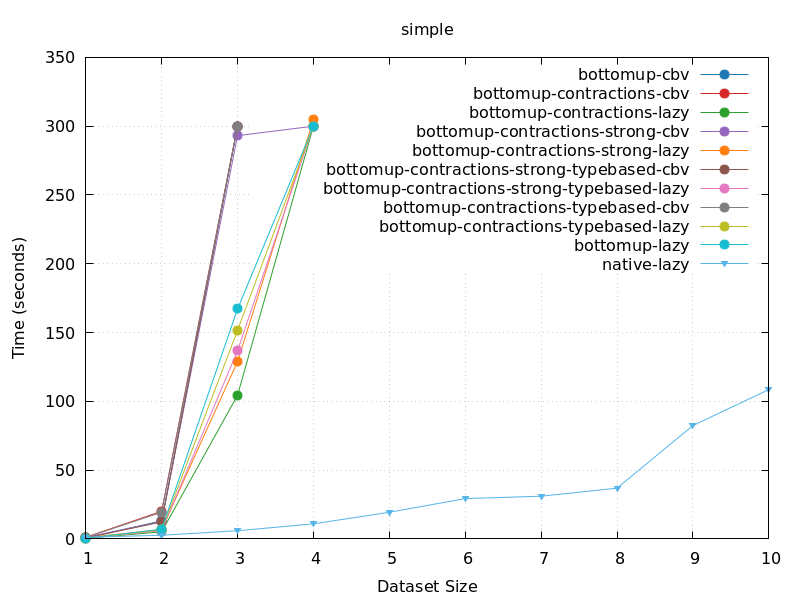
\includegraphics[width=\linewidth]{bottomup.png} 
    \caption{Семейство стратегий \texttt{bottomup-naive}}
    \end{subfigure}
    \begin{subfigure}{0.5\textwidth}
    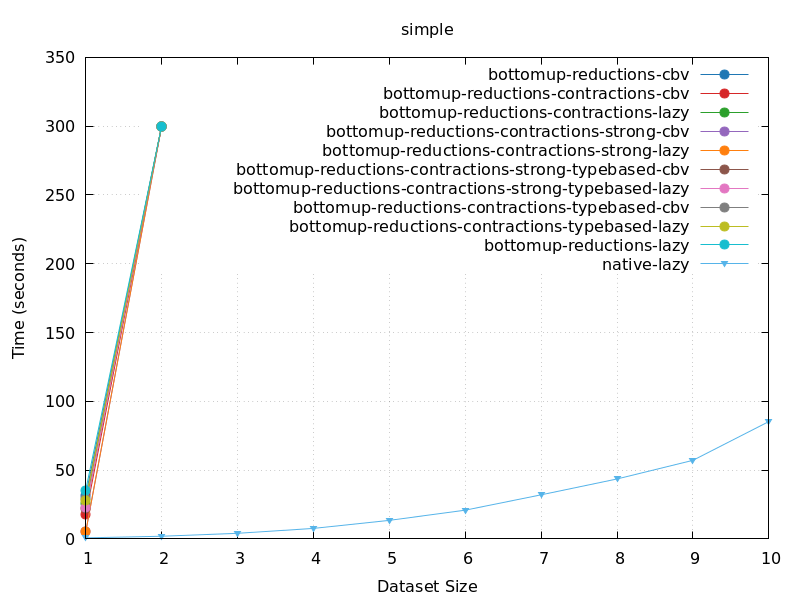
\includegraphics[width=\linewidth]{bottomup_reductions.png}
    \caption{Семейство стратегий \texttt{bottomup-reductions}}
    \end{subfigure}
    \caption{Результы сравнения стратегий \texttt{bottomup} на наборе данных Simple}
    \label{plot_bottomup}
\end{figure}

Такой резкий рост времени работы для этих стратегий, вероятно, является экспоненциальным, что несложно объяснить. Действительно, стратегия \texttt{bottomup-naive} подставляет все термы не редуцируя их, что приводит к значительной дубликации кода, и даже мемоизация в ленивом вычислении не решает проблему, поскольку ещё до запуска внутренней редукции процедура подстановки термов с дублицированным кодом становится экспоненциальной. То, что стратегия \texttt{bottomup-reductions}, включающей в себя редукции на каждом шаге, является ещё медленнее наивной версии, может показаться контринтуитивным. Однако, этот факт объясняется тем, что при преждевременной редукции термов в стратегии \texttt{bottomup-reductions}, то есть при редукции термов, которые содержат неподставленные свободные переменные $y_i$, терм может значительно увеличиваться в размерах из-за "мёртвого кода", например если такая переменная стоит в голове условного оператора или сопоставления с образцом. 

В более общем смысле, рисунок \ref{plot_bottomup} иллюстрирует, насколько важно выбрать правильный порядок вычислений и подстановок, так как в результате выбора неверного порядка легко получить стратегию, не применимую на практике из-за крайней неэффективности.


\begin{figure}[h]
    \begin{subfigure}{0.5\textwidth}
    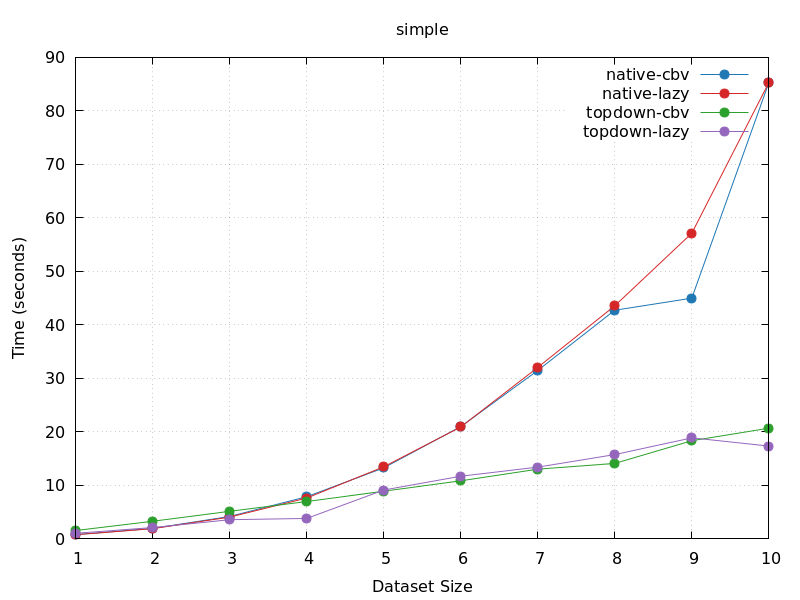
\includegraphics[width=\linewidth]{basic_simple.png} 
    \caption{Набор данных Simple}
    \end{subfigure}
    \begin{subfigure}{0.5\textwidth}
    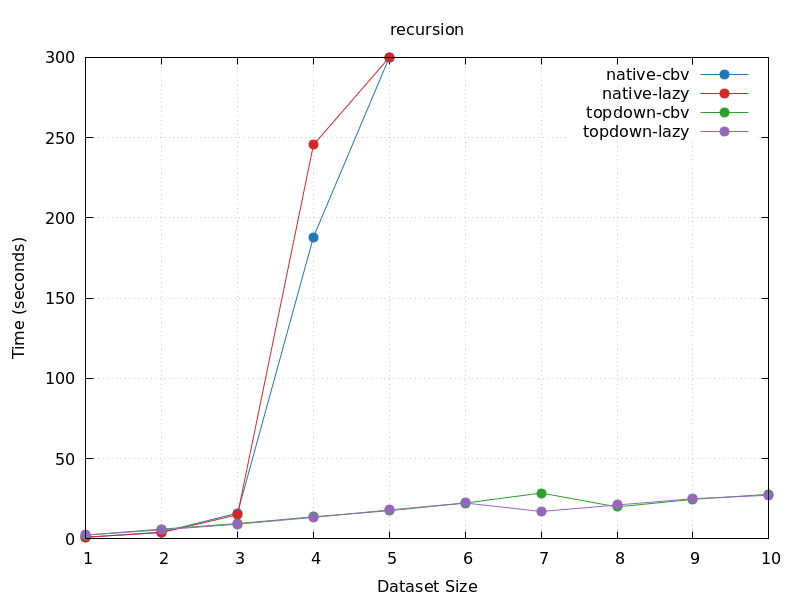
\includegraphics[width=\linewidth]{basic_recursion.png}
    \caption{Набор данных Recursion}
    \end{subfigure}
    \caption{Результаты сравнения базовых стратегий}
    \label{plot_basic}
\end{figure}

Перейдём к сравнению двух оставшихся базовых стратегий, \texttt{native} и \texttt{topdown}. Результаты сравнения этих стратегий на наборах данных Simple и Recursion приведены на рисунке \ref{plot_basic}. Оказывается, что уже базовая стратегия \texttt{topdown} показывает результаты, значительно лучше, чем \texttt{native}. На наборе данных Recursion стратегия \texttt{native} показывает экспоненциальный взрыв, похожий на наблюдаемый со стратегиями \texttt{bottomup}, и вероятно объясняемый неэффективностями в реализации редукций. Однако, стратегия \texttt{topdown} даже без дальнейших эвристических оптимизаций, использующая множество редукций для решения небольших подзадач, не демонстрирует экспоненциального поведения, и даже выглядит линейно на рассматриваемых объёмах данных. Таким образом, уже правильный выбор базовой стратегии, использующую естественную декомпозицию данных на уравнения и обрабатывающих их в необходимом порядке, позволяет значительно улучшить производительность вычислений.

Другим неожиданным наблюдением, отражённым на рисунке \ref{plot_basic}, является статистическая неразличимость при использовании внутренних редукций \texttt{cbv} или \texttt{lazy}. При наблюдении за всеми парами стратегий было не обнаружено значимой разницы при изменении этого параметра у любых стратегий. Этот факт крайне удивителен, и его причины не до конца ясны. Вероятно, это отсутствие разницы свидетельствует о неэффективности одной из редукций или о недокументированных эвристиках (напомним, что в рамках этой работы эти редукции воспринимаются как "чёрный ящик"). Однако, это наблюдение только свидетельствует о верности изначального тезиса о потребности более тонко настраивать порядок вычисления в целях оптимизации, поскольку даже одна из немногих возможностей выбора, предоставляемая встроенными инструментами Coq, не оказывает серьёзного влияния на эффективность вычислений. В дальнейших графиках и рассуждениях выбор внутренней редукции будет опускаться (конкретнее, во всех данных будет использоваться версия \texttt{lazy} для всех стратегий).

Итак, стратегия \texttt{topdown} уже показывает значительное, асимптотическое улучшение относительно стратегии \texttt{native}, что является центральным практическим результатом работы. Однако, можно получить ещё более эффективные стратегии, рассмотрев дальнейшие эвристики, описанные в разделах \ref{graphbased} и \ref{typebased}. Результаты сравнения этих стратегий приведены на рисунке \ref{plot_heuristics}.

\begin{figure}[h]
    \begin{subfigure}{0.5\textwidth}
    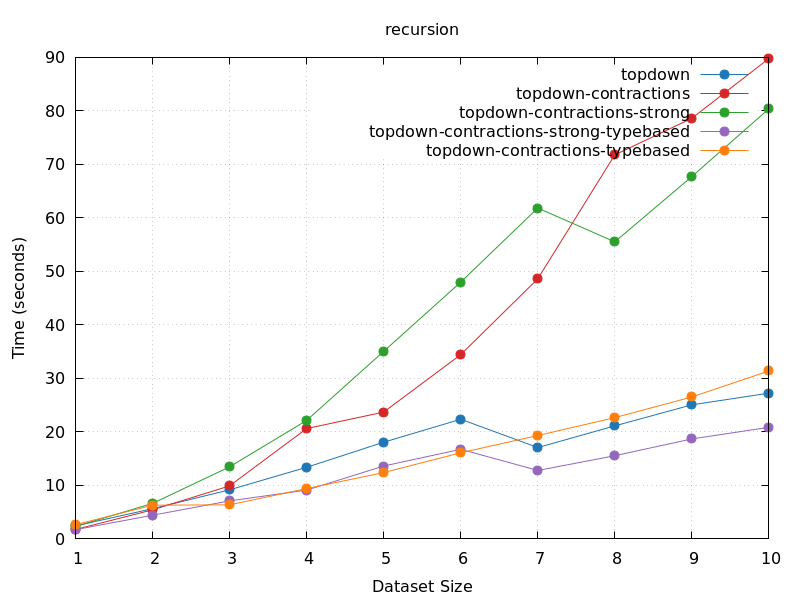
\includegraphics[width=\linewidth]{topdown.png} 
    \caption{Семейство стратегий \texttt{topdown}}
    \label{plot_heuristics_topdown}
    \end{subfigure}
    \begin{subfigure}{0.5\textwidth}
    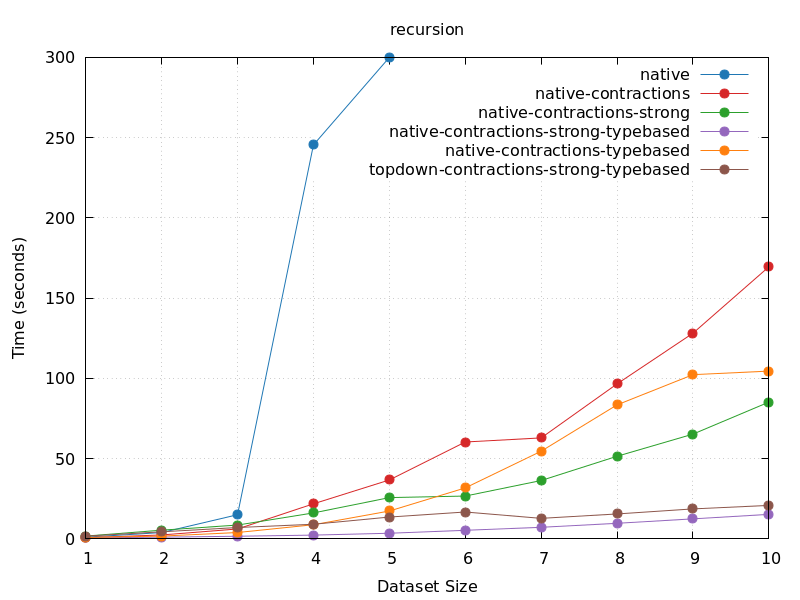
\includegraphics[width=\linewidth]{native.png}
    \caption{Семейство стратегий \texttt{native}}
    \label{plot_heuristics_native}
    \end{subfigure}
    \caption{Результаты сравнения стратегий с эвристическими оптимизациями на наборе данных Recursion}
    \label{plot_heuristics}
\end{figure}

Рассматривая результаты различных эвристических оптимизаций стратегии \\\texttt{topdown} (рис. \ref{plot_heuristics_topdown}), можно заметить, что почти все из них оказывают негативное влияние на производительность. Так, хуже всего результат показывают оптимизации, основанные на чистых графовых свойствах (\texttt{topdown-contractions} и \\\texttt{topdown-contractions-strong}), из-за накладных расходов на явное построение графа они проигрывают базовой стратегии. Не показывает значительного улучшения и слабая версия оптимизации, основанной на типах данных \texttt{topdown-contractions-} \texttt{typebased}. Однако сильная версия этой оптимизации \texttt{topdown-contractions-strong-} \texttt{typebased} немного быстрее, чем базовая версия \texttt{topdown}.

Что же касается тех же оптимизаций, применённых для стратегии \texttt{native} (рис. \ref{plot_heuristics_native}), то они все улучшают эффективность базовой стратегии и не показывают такого резкого роста. Однако, их относительный порядок совпадает с изложенным для \texttt{topdown}, а именно графовые эвристики и слабая версия типовой эвристики показывают не такой эффективный результат, как сильная версия типовой эвристики \texttt{native-contractions-strong-typebased}. Интересно, что несмотря на то, что базовая версия \texttt{native} значительно медленнее базовой версии \texttt{topdown}, если применить к обеим стратегиям оптимизацию \texttt{contractions-strong-typebased}, то \texttt{native} станет даже немного, но статистически заметно, эффективнее \texttt{topdown}.

Итак, выявлены три стратегии, показывающие наилучшие результаты: стратегия \texttt{topdown} в базовой версии и стратегии \texttt{topdown} и \texttt{native} с оптимизацией \texttt{contractions-} \texttt{strong-typebased}. На рисунке \ref{plot_winners} приведены результаты этих трёх стратегий на больших объёмах данных (до n = 40, тогда как предыдущие графики включали данные до n = 10). 

\begin{figure}[h]
    \begin{subfigure}{0.5\textwidth}
    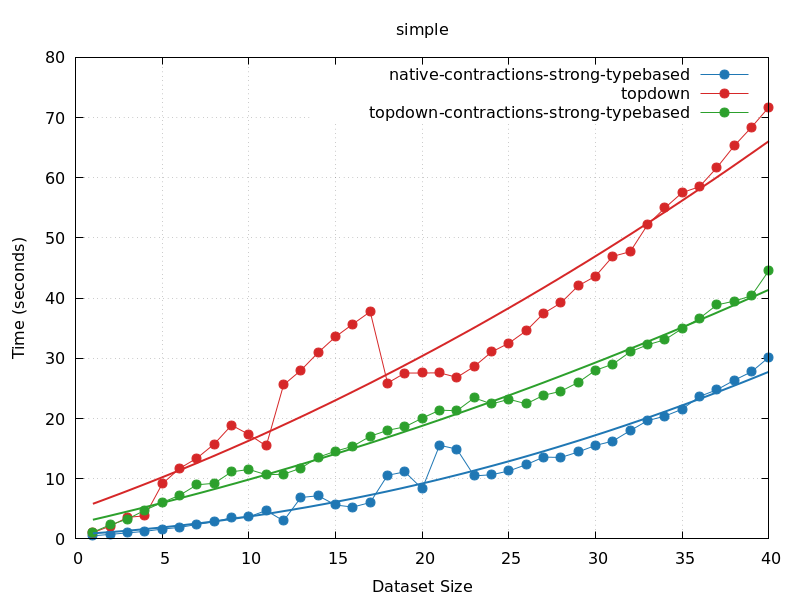
\includegraphics[width=\linewidth]{winners_simple.png} 
    \caption{Набор данных Simple}
    \label{plot_winners_simple}
    \end{subfigure}
    \begin{subfigure}{0.5\textwidth}
    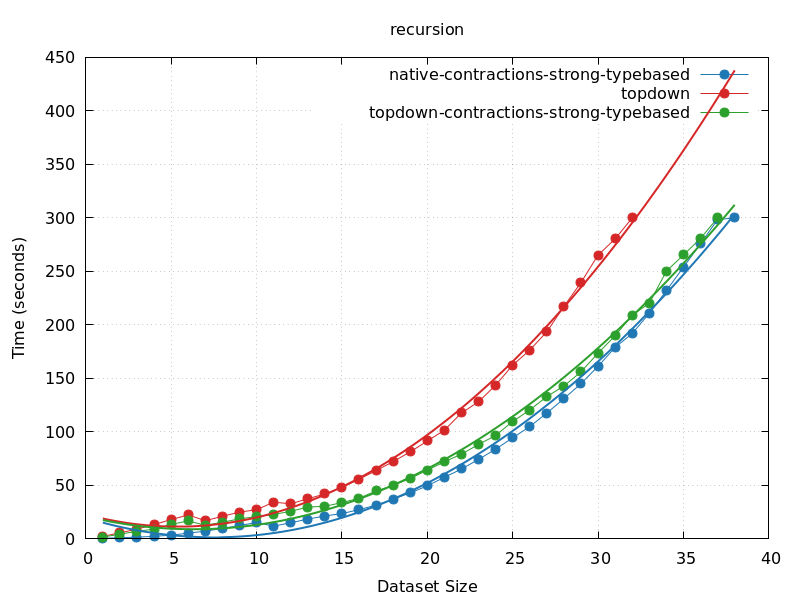
\includegraphics[width=\linewidth]{winners_recursion.png}
    \caption{Набор данных Recursion}
    \label{plot_winners_recursion}
    \end{subfigure}
    \caption{Результаты сравнения лучших стратегий на больших данных с линией тренда}
    \label{plot_winners}
\end{figure}

На наборе данных Simple (рис. \ref{plot_winners_simple}) рост стратегий выглядит почти линейным, кривизна графика не очень заметна. Однако, на наборе данных Recursion (рис. \ref{plot_winners_recursion}), который является в несколько раз более вычислительно затратным по размеру системы уравнений, чем набор Simple, отчётливо видно, что рост всех трёх стратегий несёт квадратичный характер. Несмотря на то, что было бы предпочтительнее получить линейный алгоритм, коэффициэнты этого квадратичного роста достаточно малы и приемлимы на практике. Так, за пять минут лучшая стратегия может обработать линейный код из нескольких сотен [TODO сколько именно?] строк кода с глубиной рекурсии до 35, что соответствует реалиям разработки смарт-контрактов. Отметим, что стратегия \texttt{native} без оптимизаций за пять минут может обработать только линейный код из нескольких десятков [TODO сколько именно?] строк кода с глубиной рекурсии до 4, то есть существенно меньше, и не может обрабатывать за адекватное время большую часть реальных смарт-контрактов.

На всех рассматриваемых наборах данных эффективнее всего проявляет себя стратегия \texttt{native-contractions-strong-typebased}, хотя её преимущество относительно стратегии \texttt{topdown-contractions-strong-typebased} не очень велико на больших тестах. Что же касается преимущества относительно базовой стратегии \texttt{topdown}, то есть преимущества стратегии с эвристическими оптимизациями перед лучшей базовой стратегией, оно также может показаться незначительным на больших тестах, поскольку асимптотического выигрыша эвристические оптимизации не привносят и на больших тестах разница между ними не кажется существенной. Однако, на вполне реалистичных размерах функции в 70 строк (n = 35 в наборе данных Simple) и глубине рекурсии в 10, эвристические оптимизации позволяют ускорить вычисление в 3 раза. Такие оптимизации могут быть особенно значимы в случаях, когда символьное вычисление используется в композитных процессах, например при доказательстве свойств сложных сценариев, где этот множитель 3 будет возведён в степень. Таким образом, несмотря на то, что уже базовая стратегия \texttt{topdown} показывает хороший результат, результат дальнейших оптимизаций также значим на практике.

TODO результаты с условными операторами

\subsection{Эксперименты на реальных данных}

TODO

\subsection{Выводы и результаты по главе}

Создан тестовый набор из синтетической части (четыре программы на языке Ursus линейно растущего размера, покрывающие фундаментальные конструкции языков программирования) и реальной части (смарт-контракт из практики компании Pruvendo). По результатам экспериментов с запуском стратегий на тестах можно сделать следующие выводы:

\begin{itemize}
    \item все стратегии класса \texttt{bottomup} экспоненциальны и неприменимы на практике; 
    \item выбор между внутренними редукциями \texttt{lazy} и \texttt{cbv} не оказывает значительного эффекта; 
    \item базовая стратегия \texttt{topdown} уже значительно эффективнее, чем \texttt{native}; 
    \item графовые эвристики и слабая версия эвристики на типах данных оказывает отрицательное влияние или незначительное положительное влияние на эффективность стратегий;
    \item лучшие результаты показывают стратегии \texttt{native} и \texttt{topdown} с применённой эвристикой \texttt{contractions-strong-typebased}, они растут квадратично, так же как и базовая стратегия \texttt{topdown}, но демонстрируют значительное неасимптотическое улучшение относительно базовой стратегии.
\end{itemize}

\end{document}
